\section{Introduction}
\label{introduction}

In the last 10 years GPUs computing has transformed the high performance 
computing, machine learning, and data analytics fields that were previously 
dominated by CPU-based 
installations~\cite{intersect360,cudnn,Lavin15b,SimonyanZ14a}. Many systems now 
rely on a combination of GPUs and CPUs to leverage high throughput data parallel 
GPUs with latency critical execution occurring on the CPUs. In part, 
GPU-accelerated computing has been successful in these domains because of native 
support for data parallel programming languages~\cite{CUDA7,OPENCL} that reduce 
programmer burden when trying to scale programs across ever growing data sets.

\begin{figure}[t]
\centering
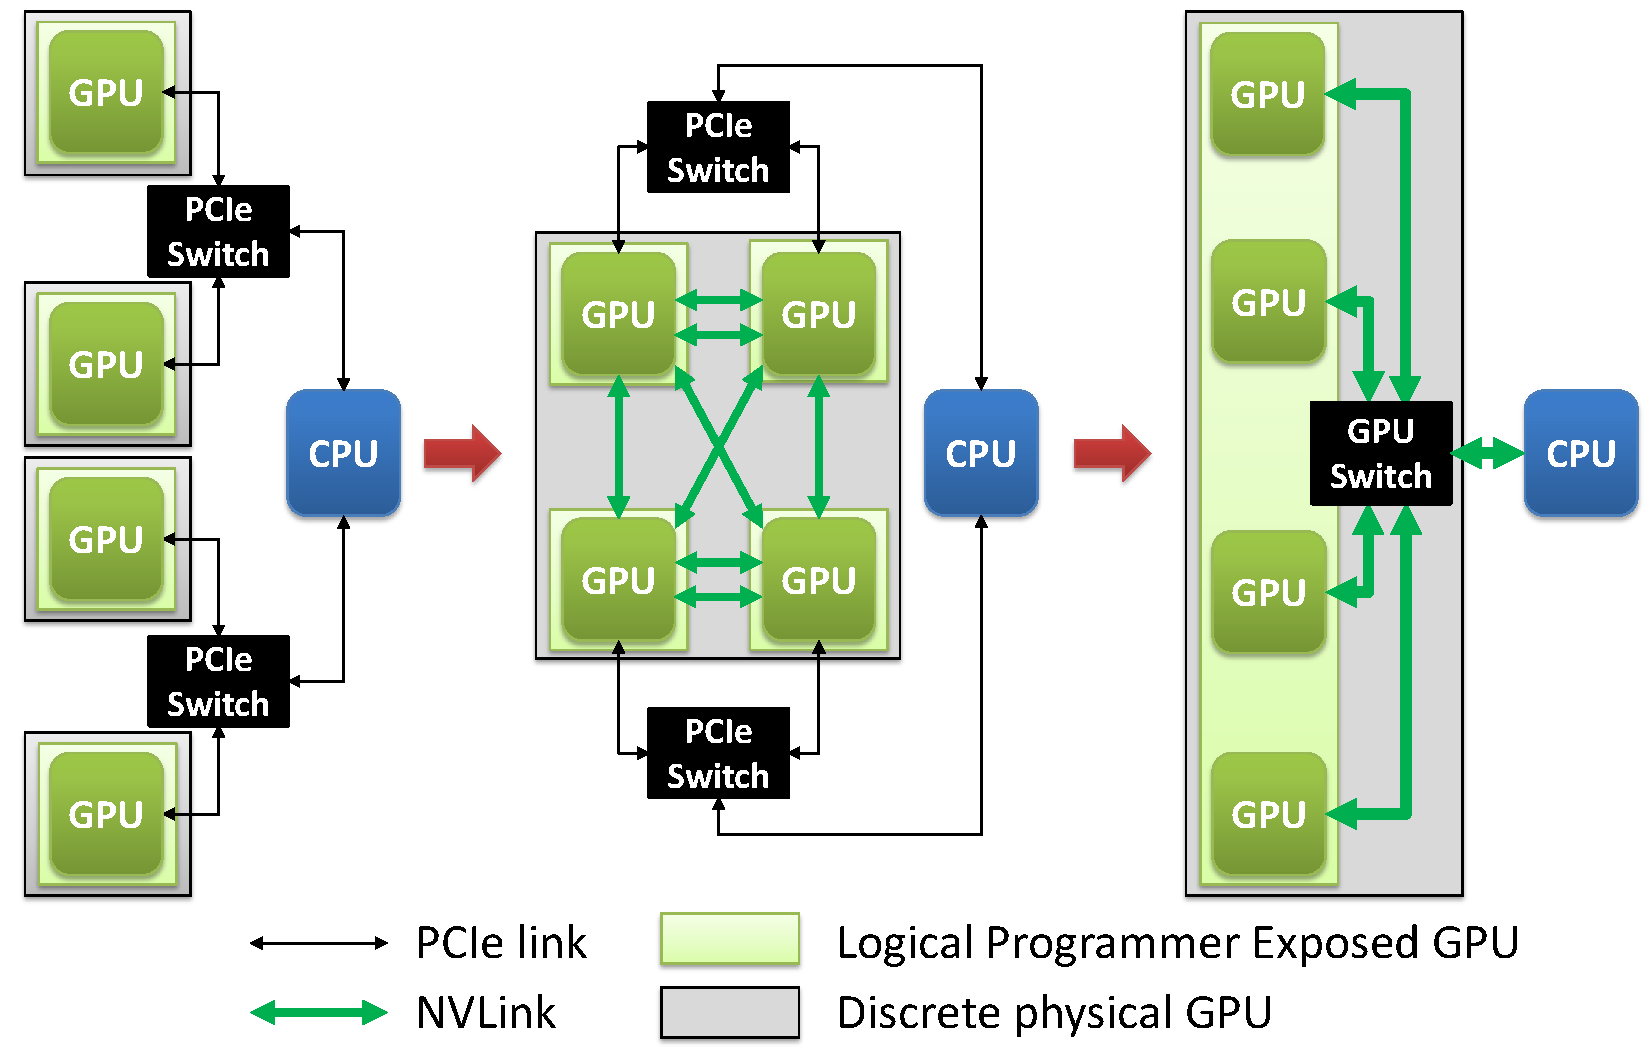
\includegraphics[width=1.0\columnwidth]{figures/inter_gpu_connections.pdf}
\caption{The evolution of GPUs from multiple discrete PCIe devices to 
single logical, multi-socket accelerators utilizing switched interconnects.}
\label{fig:systemdiagram}
\vspace{-.2in}
\end{figure}

Nevertheless, with GPUs nearing the reticle limitation for maximum die size and 
the transistor density growth rate slowing down~\cite{mooredead2016}, developers 
looking to scale the performance of their single GPU programs are in a 
precarious position. Multi-GPU programming models support explicit programming 
of two or more GPUs, but it is challenging to leveraging mechanisms such as 
Peer-2-Peer access~\cite{NVIDIAP2P} or a combination of MPI and 
CUDA~\cite{NVIDIAMPI} to manage multiple GPUs. These programming extensions 
enable programmers to employ more than one GPU for high throughput computation, 
but they require re-writing of traditional single GPU applications which has 
slowed their adoption rate.

Recently GPUs have started to expand beyond the traditional PCIe
peripheral interface to enable a single protocol interconnection
between both the GPUs and CPUs~\cite{dgx,SierraHPC,AMDINFINITYFABRIC},
as shown in Figure~\ref{fig:systemdiagram}.  As a result, some GPUs
are being delivered on high pin-count socketed modules to provide
high-speed links for interconnect bandwidth that is up to an order of
magnitude higher than PCIe connections.  The expansion of GPUs from
single pluggable devices to closely coupled multi-socket designs is a
natural progression as GPU--GPU and CPU--GPU link bandwidth becomes a
performance critical system component.

The onset of multi-socket GPUs provides a pivot point for GPU and system 
vendors. On one hand, vendors can continue to expose multi-socket GPUs as 
individual GPUs and force developers of multi-GPU systems to use multiple
programming paradigms to 
leverage multiple GPUs. On the other, vendors could expose multi-socket 
designs as a single non-uniform memory access (NUMA) GPU resource.  By 
extending the single GPU programming model to multi-socket GPUs,  applications 
can scale beyond the bounds of Moore's law, while simultaneously retaining the 
programming interface that GPU developers have become accustomed.

Several groups have previously examined aggregating multiple GPUs together under 
a single programming model~\cite{lee2013transparent,Cabezas2015}; however this 
work was done in an era where GPUs had limited memory addressability and relied 
on high latency, low bandwidth PCIe interconnects. As a result, prior work 
focused primarily on improving the multi-GPU programming experience rather than 
achieving highly scalable performance. Building upon this work, we propose a 
multi-socket \textit{NUMA-aware} GPU architecture and runtime that aggregates 
multiple GPUs into a single programmer transparent logical GPU. We show that in 
the the era of unified virtual addressing~\cite{UVM}, cache line addressable 
high bandwidth interconnects~\cite{NVLINK}, and dedicated GPU and CPU socket PCB 
designs~\cite{SierraHPC}, scalable multi-GPU performance may be achievable under 
existing single GPU programming models. In this work, we make the following 
contributions:

\begin{itemize}

\item We show that traditional software NUMA memory placement and 
scheduling policies are not sufficient for multi-socket GPUs to achieve 
performance scalability.  We then demonstrate that intersocket bandwidth will be 
the primary performance limiter in future NUMA GPUs.

\item By exploiting program phase behavior we show that intersocket links (and 
thus BW) should be dynamically varied at runtime to maximize link 
utilization. Moreover, we show that link policy must be determined on a per 
GPU basis, as global policies fail to capture per GPU phase behavior.

\item We show that both the GPU L1 and L2 caches should be made NUMA-aware 
and dynamically adapt their caching policy to minimize NUMA effects. We demonstrate
that in NUMA GPUs, extending existing GPU cache coherence protocols
across multiple sockets scales is a good design choice, despite the overheads.

\item We show that multi-socket NUMA-aware GPUs can allow traditional 
GPU programs to scale efficiently to as many as 8 GPU sockets, providing significant 
headroom before developers must re-architect applications to obtain additional performance.

\end{itemize}
